\documentclass{article}
\usepackage{tikz}

\begin{document}

\begin{figure}[h]
    \centering
    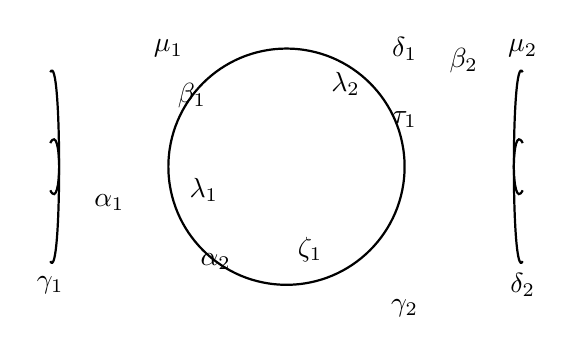
\begin{tikzpicture}[scale=1.5]
        % Draw the circular part of the mesh
        \draw[thick] (0,0) circle (1);
        
        % Draw the curved part of the mesh
        \draw[thick] (-2,-0.2) .. controls (-1.9, -0.4) and (-1.9, 0.4) .. (-2,0.2);
        \draw[thick] (-2,-0.8) .. controls (-1.9,-1) and (-1.9,1) .. (-2,0.8);
        \draw[thick] (2,-0.8) .. controls (1.9,-1) and (1.9,1) .. (2,0.8);
        \draw[thick] (2,-0.2) .. controls (1.9,-0.4) and (1.9, 0.4) .. (2,0.2);
        
        % Label the parts of the mesh
        \node at (-1,1) {$\mu_{1}$};
        \node at (-2,-1) {$\gamma_{1}$};
        \node at (1,1) {$\delta_{1}$};
        \node at (-0.8, 0.6) {$\beta_{1}$};
        \node at (-1.5, -0.3) {$\alpha_{1}$};
        \node at (-0.7, -0.2) {$\lambda_{1}$};
        \node at (1,0.4) {$\tau_{1}$};
        \node at (0.2, -0.7) {$\zeta_{1}$};
        \node at (-0.6, -0.8) {$\alpha_{2}$};
        \node at (1.5, 0.9) {$\beta_{2}$};
        \node at (2,1) {$\mu_{2}$};
        \node at (2,-1) {$\delta_{2}$};
        \node at (1,-1.2) {$\gamma_{2}$};
        \node at (0.5, 0.7) {$\lambda_{2}$};
    \end{tikzpicture}
    \caption{Left: Partial and whole spherical linkage of a mesh in Fig. \ref{sqmesh}. The segments labeled as $(\lambda_{i}, \gamma_{i}, \mu_{i}, \delta_{i}, \alpha_{i}, \beta_{i})$ and $(\lambda_{i}', \gamma_{i}', \mu_{i}', \delta_{i}', \alpha_{i}', \beta_{i}')$ are complementary to $\pi$. The gap between $\beta_{1}$ and $\alpha_{2}$ is due to the overlapping segments $\tau_{1}$ and $\zeta_{1}$.}
    \label{sqmesh}
\end{figure}

\end{document}